
\chapter{Android aplikacija}

\section{Arhitektura}

Napravljena Android aplikacija ima sljede\'{c}e uvjete za ure\dj aje na kojima se mo\v{z}e pokrenuti:

\begin{itemize}
		\item Minimalna verzija Android operativnog sustava je 5.0. (Android SDK verzija 21, kodnog naziva Lollipop)
		\item NFC modul
		\item BLE modul
\end{itemize}

\subsection{MVP}

Aplikacija je implementirana prema Model View Presenter (MVP) oblikovnom obrascu \cite{mvp}. Svrha ovog obrasca je logi\v{c}ki strukturirati aplikaciju na na\v{c}in da se prezentacijski sloj odvoji od poslovne logike aplikacije. Prezentacijski sloj uklju\v{c}uje korisni\v{c}ko su\v{c}elje i sve \v{s}to korisnik vidi, \v{c}uje ili osjeti pomo\'{c}u pametnog telefona, dok poslovna logika uklju\v{c}uje dohva\'{c}anje i obradu podataka koji se prikazuju na su\v{c}elju te op\'{c}enito svu logiku koju aplikacija implementira. Razlog uvo\dj enja slojeva i odvajanja logike od prezentacijskog dijela je kreacija odr\v{z}ivog sustava koji je jednostavno nadograditi i testirati. Prednost je i to \v{s}to je kod strukturiran i \v{c}itljiv, \v{s}to olak\v{s}ava rad vi\v{s}e ljudi na istom projektu i njegovo odr\v{z}avanje.

Na slici ~\ref{fig:mvp} je prikazana shema komunikacije izme\dj u slojeva u MVP oblikovnom obrascu.

\begin{figure}[!htbp]
	\begin{center}
 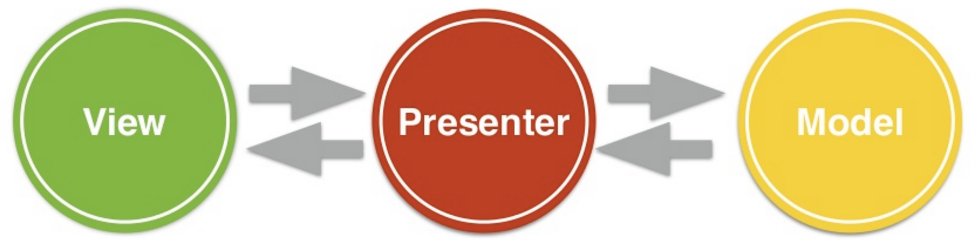
\includegraphics[height=3.5cm,keepaspectratio=true]{mvp}
 \caption{Komunikacija slojeva u MVP oblikovnom obrascu}
 \label{fig:mvp}
	\end{center}
\end{figure}

Sloj View je jedini sloj s kojim korisnik ima direktnu interakciju. On ima za zada\'{c}u prikazati podatke na korisni\v{c}kom su\v{c}elju i reagirati na sve korisni\v{c}ke interakcije (npr. odabir elementa liste, dodir gumb...). View u sebi posjeduje referencu na Presenter i njegova uloga je zapravo pozivati odgovaraju\'{c}e metode Presentera nakon \v{s}to se dogodi odre\dj ena akcija i prikazivanje podataka koje mu Presenter proslijedi.

Sloj Presenter sadr\v{z}i glavnu logiku Android aplikacije iz razloga \v{s}to je posrednik izme\dj u View i Model sloja. On odlu\v{c}uje kako reagirati na neku korisnikovu akciju, na koji na\v{c}in dohvatiti podatke iz Model sloja i op\'{c}enito odre\dj uje cijelo korisni\v{c}ko iskustvo sa aplikacijom.

Sloj Model je zadu\v{z}en za dohva\'{c}anje podataka (iz interne memorije ure\dj aja, baze podataka aplikacije ili internetskog poslu\v{z}itelja) i serijaliziranje istih u modele koji se koriste u ostatku aplikacije. Iz tog razloga se dijeli na dva dijela: interactor (vr\v{s}i interakciju sa podacima) i same modele (Java klase).

MVP se na Android platformi, u programskom jeziku Java, implementira uz pomo\'{c} su\v{c}elja u kojima su definirani prototipi metoda koje klasa koja implementira su\v{c}elje mora implementirati. Ovaj na\v{c}in podi\v{z}e razinu apstraktnosti i dopu\v{s}ta programeru da prvo dobro logi\v{c}ki osmisli najbolji na\v{c}in za napraviti MVP sa datim zahtjevima, s ciljem maksimiziranja efekata obrasca, a zatim da se posveti i samoj implementaciji. Na slici ~\ref{fig:mvp} je na primjeru dohva\'{c}anja konfiguracije poslovnice prikazana implementacija MVP obrasca u napravljenoj Android aplikaciji.


\begin{figure}[!htbp]
	\begin{center}
 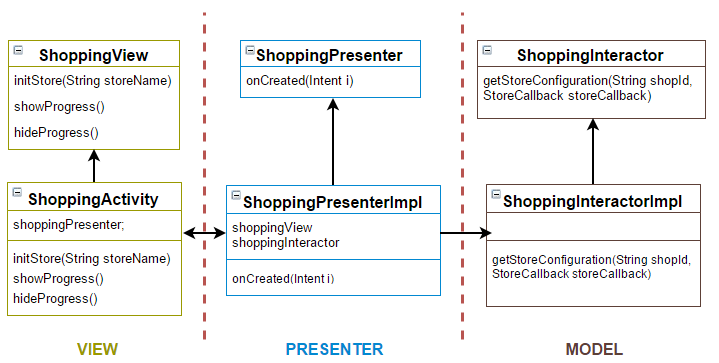
\includegraphics[height=7.5cm,keepaspectratio=true]{mvp_primjer}
 \caption{Primjer MVP-a u napravljenoj aplikaciji}
 \label{fig:mvp}
	\end{center}
\end{figure}

Slika ~\ref{fig:mvp} prikazuje tijek doga\dj aja od trenutka kada korisnik skenira NFC naljepnicu do trenutka kada mu se prikazuje su\v{c}elje za poslovnicu u kojoj se nalazi. Klasa ShoppingActivity je Java klasa koja pro\v{s}iruje klasu Activity (aktivnost), koja dolazi sa Android SDK-om. Aktivnost je najlak\v{s}e tuma\v{c}iti kao jedan zaslon aplikacije, te ShoppingActivity predstavlja zaslon koji je korisniku predstavljen u trenutku kada se on nalazi u poslovnici te je u potrazi za popustima.

U trenutku kada korisnik skenira NFC naljepnicu pokre\'{c}e se aktivnost ShoppingActivity (u poglavlju 3.1.2 ``Pasivna komunikacija'' je detaljno opisan mehanizam koji ovo omogu\'{c}uje). Ona implementira ShopingView su\v{c}elje i ima referencu na ShoppingPresenterImpl objekt koji implementira ShoppingPresenter, kojem zove metodu onCreated(Intent i). ShoppingPresenterImpl tada iz objekta Intent i \v{c}ita identifikacijski broj poslovnice te je spreman inicirati zahtjev za dohva\'{c}anje podataka o poslovnici sa poslu\v{z}itelja. Prvo zove metodu showProgress() (implementirana u aktivnosti ShoppingActivity) koja slu\v{z}i da bi se korisniku prikazao ProgressDialog (mehanizam koji korisniku prikazuje indikator da pri\v{c}eka jer se neka operacija izvr\v{s}ava, prikazan je na slici ~\ref{fig:progressDialog}). Zatim zove interaktorovu metodu getStoreConfiguration() (implementiranu u klasi ShoppingInteractor) kojoj predaje identifikaciju poslovnice i objekt koji implementira su\v{c}elje StoreCallback.


\begin{figure}[!htbp]
	\begin{center}
 
\includegraphics[height=3cm,keepaspectratio=true]{progressDialog}
 \caption{ProgressDialog koji korisniku daje do znanja da mora pri\v{c}ekati jer se neka operacija obavlja u pozadini}
 \label{fig:progressDialog}
	\end{center}
\end{figure}

Metoda getStoreConfiguration() kreira poslu\v{z}iteljski zahtjev za konfiguracijom poslovnice. Praksa je da se zahtjev izvr\v{s}ava na novoj dretvi iz razloga \v{s}to se vrijeme potrebno poslu\v{z}itelju za odgovor ne mo\v{z}e unaprijed znati, te nema smisla da glavna dretva aplikacije zbog toga bude blokirana, jer to rezultira zamrznutim ekranom telefona \v{s}to stvara neugodno korisni\v{c}ko iskustvo. Zbog navedenog razloga, interaktoru se \v{s}alje objekt storeCallback koji implementira su\v{c}elje StoreCallback prikazano na slici ~\ref{fig:storeCallback}, koje definira metodu za uspjeh i neuspjeh zahtjeva. Ukoliko je zahtjev uspio, interaktor serijalizira dobivene podatke u odgovaraju\'{c}i model (serijalizacija je potrebna jer poslu\v{z}itelj vra\'{c}a podatke u JSON formatu) kojeg preko su\v{c}elja \v{s}alje nazad prezenteru. Ukoliko zahtjev nije uspio (npr. poslu\v{z}itelj nije aktivan ili telefon nema pristup internetu), zove se metoda za neuspjeh koja za krajnji cilj ima korisniku prikazati da je do\v{s}lo do gre\v{s}ke.


\begin{figure}[!htbp]
	\begin{center}
 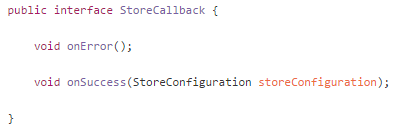
\includegraphics[height=3cm,keepaspectratio=true]{storeCallback}
 \caption{Su\v{c}elje StoreCallback sa prototipima metoda za uspjeh i neuspjeh zahtjeva za konfiguracijom poslovnice.}
 \label{fig:storeCallback}
	\end{center}
\end{figure}

Prvo \v{s}to prezenter napravi nakon \v{s}to dobije interaktorov odgovor je skrivanje ProgressDialog-a na na\v{c}in da pozove metodu hideProgress() u aktivnosti. Nakon toga, inicijalizira su\v{c}elje sa informacijama o poslovnici te kao vlastiti atribut sprema listu popusta, koje evaluira nakon \v{s}to mu aktivnost javi da je BLE ogla\v{s}iva\v{c} prona\dj en, na isti na\v{c}in kao \v{s}to javlja da je korisnik u\v{s}ao u poslovnicu. Sva logika aplikacije je implementirana na istim principima MVP-a, \v{s}to je \v{c}ini mnogo \v{c}itljivijom i bolje organiziranom od toga da je sve implementirano u klasi aktivnosti.

\subsection{NFC komunikacija}

Za potrebe ovog projekta implementirana je jednosmjerna NFC komunikacija izme\dj u pametnog telefona i NFC naljepnice. Zahtjev projekta uklju\v{c}uje pokretanje aktivnosti za tra\v{z}enje popusta prilikom skeniranja NFC naljepnice u odre\dj enoj poslovnici. To je omogu\'{c}eno pomo\'{c}u mehanizma u Android operativnom sustavu koji zapo\v{c}inje instalacijom aplikacije na pametni telefon. Prilikom instalacije Android analizira sadr\v{z}aj datoteke AndroidManifest \cite{androidManifest} u kojoj su specificirane najva\v{z}nije informacije o aplikaciji, koje me\dj u ostalim uklju\v{c}uju: ime paketa aplikacije, popis svih aktivnosti u aplikaciji, dozvole koje aplikacija zahtjeva (npr. NFC, BLE, kamera, mikrofon). Prilikom definiranja aktivnosti aplikacije, mogu\'{c}e je definirati da je odre\dj ena aktivnost sposobna obraditi odre\dj enu vrstu podataka. Ti podaci su objekti klase Intent (eng. namjera, klasa definirana u Android SDK-u) te sadr\v{z}e opis akcije koja se treba izvr\v{s}iti i dodatne podatke. Kod instaliranja nove aplikacije, operativni sustav u svoju internu memoriju zapisuje aktivnosti koje su sposobne za obradu odre\dj ene vrste Intenta. Kada tokom kori\v{s}tenja telefona do\dj e do zahtjeva za Intentom, Android provjeri koje aplikacije mogu obraditi taj intent i korisniku prika\v{z}e izbornik u kojem odabire \v{z}eljenu aplikaciju (mo\v{z}e se definirati i predodre\dj ena aplikacija pa se izbornik ne\'{c}e prikazivati).

Ozna\v{c}avanje aktivnosti kao sposobne za obraditi Intent se radi pomo\'{c}u Intent filtera, u kojem se obavezno mora specificirati ime akcije. Na slici \ref{fig:intentFilter} je prikazan zapis iz AndroidManifet-a za aktivnost koja sadr\v{z}i logiku za \v{c}itanje NFC naljepnica namijenjenih za ovu aplikaciju, koja uklju\v{c}uje odgovaraju\'{c}i Intent filter.

\begin{figure}[!htbp]
	\begin{center}
 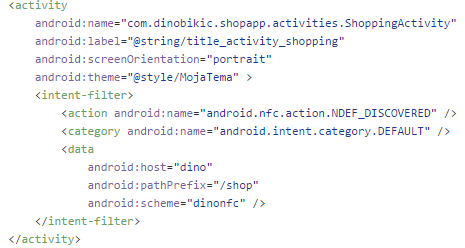
\includegraphics[height=6cm,keepaspectratio=true]{intentFilter}
 \caption{Primjer definiranja aktivnosti sa IntentFilter-om u AndroidManifest-u}
 \label{fig:intentFilter}
	\end{center}
\end{figure}

Kada korisnik uklju\v{c}i NFC modul na svome ure\dj aju, Android u pozadini skenira okolinu pomo\'{c}u NFC senzora te kada nai\dj e na NFC ure\dj aj kreira Intent objekt s akcijom koja ovisi o vrsti podacima zapisanim na NFC ure\dj aju. Za potrebe projekta, sve NFC naljepnice su morale imati u svojoj memoriji zapisan Uniform Resource Identifier (URI) u kojem je specificirano ime paketa aplikacije koja obra\dj uje pro\v{c}itane podatke i identifikacija poslovnice. Takvi NFC ure\dj aji su prema NFC Forum-u specificirani kao NDEF \cite{NdefMessage} (Android naziva akciju nala\v{z}enja ovakvih ure\dj aja \verb|NDEF_DISCOVERED| \cite{ndef_discovered}).
Stoga, ovakva konfiguracija za rezultat ima pokretanje aktivnosti ShoppingActivity pri skeniranju NFC naljepnice. ShoppingActivity tada \v{s}alje cijeli Intent objekt u prezenter koji \v{c}ita vrijednost skenirane naljepnice te radi zahtjev za konfiguracijom poslovnice u kojoj se korisnik nalazi.

\subsubsection{Priprema NFC naljepnice}
Za zapis podataka na naljepnicu je kori\v{s}tena aplikacija NFC Tools \cite{nfcTools}. Aplikacija ima pla\'{c}enu i besplatnu verziju, a za potrebe projekta je bila dovoljna besplatna verzija preko koje se sa naljepnice mogu \v{c}itati i zapisivati podaci. Proces zapisivanja URI-a je prikazan na slici \ref{fig:zapisNfca}.


\begin{figure}[!htbp]
	\begin{center}
 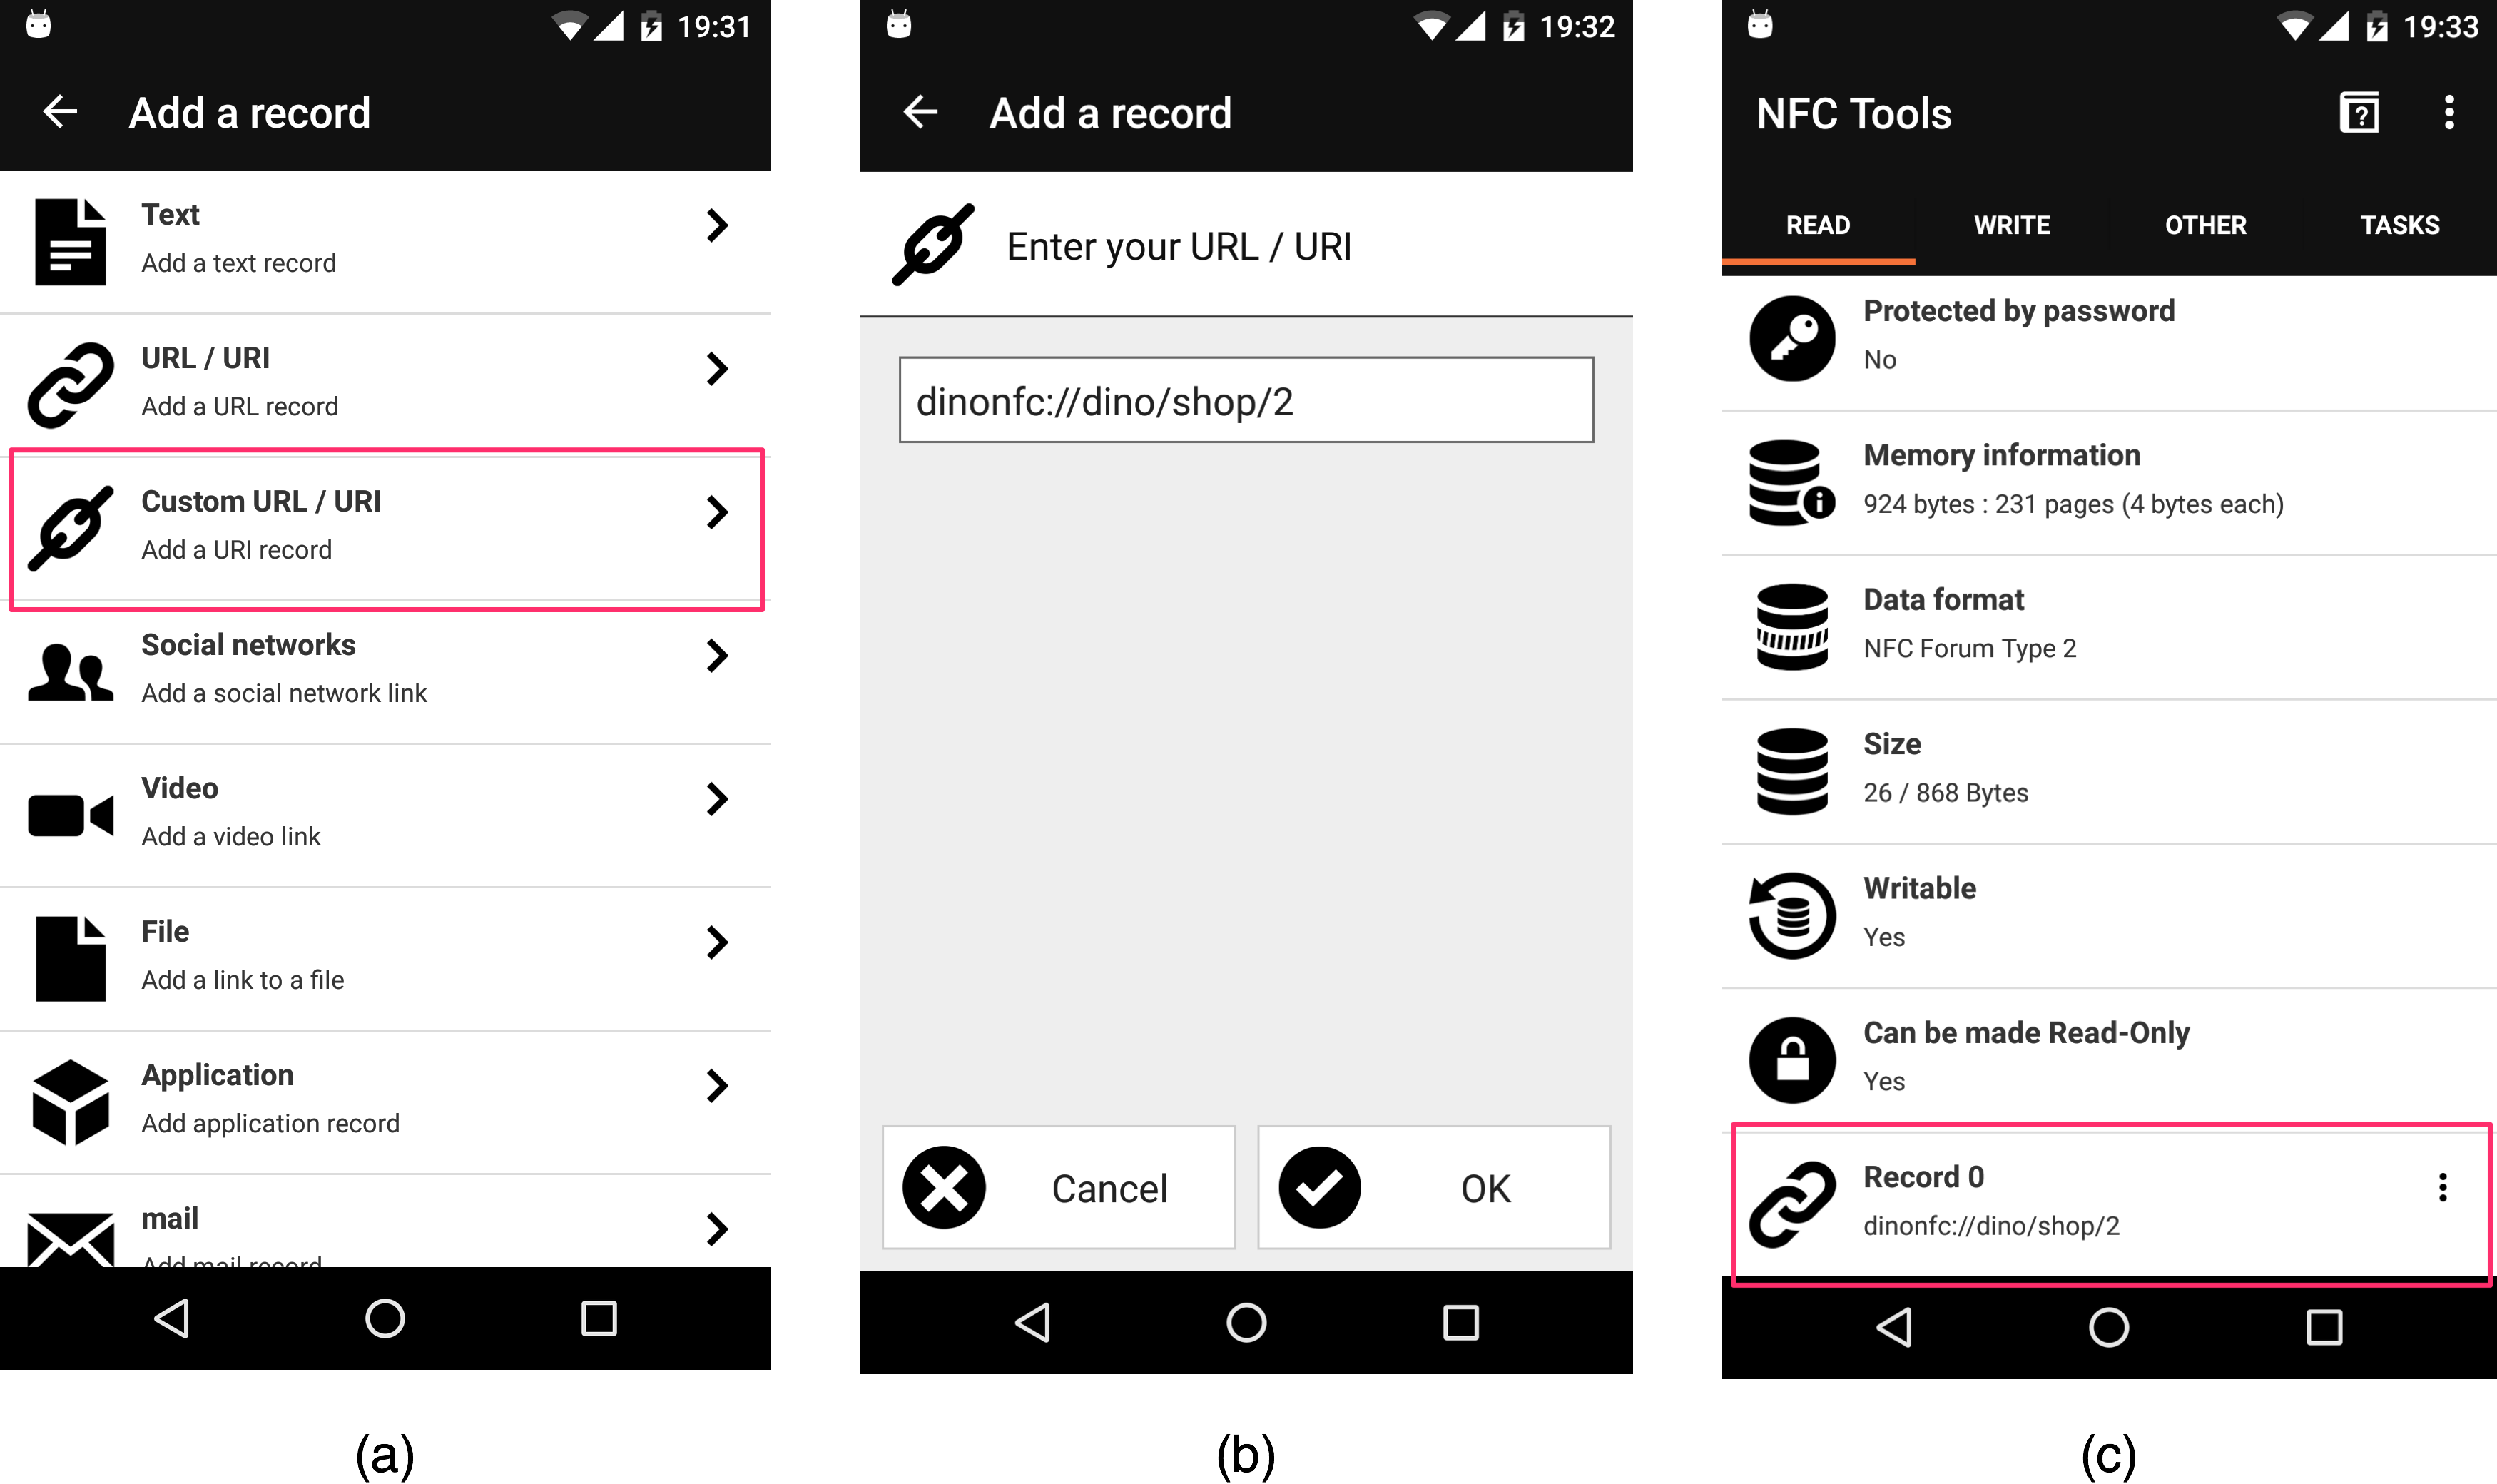
\includegraphics[height=9cm,keepaspectratio=true]{zapis_nfca}
 \caption{Na slici je prikazan proces zapisivanja URI-a na NFC naljepnicu. Ekran (a) prikazuje odabir zapisivanja URI-a, ekran (b) prikazuje upisivanje URI-a. Nakon \v{s}to je URI upisan potrebno je prisloniti naljepnicu na pametni telefon, s ciljem zapisivanja podataka. Ekran (c) prikazuje pro\v{c}itani zapis naljepnice kojoj smo prethodno zapisali URI.}
 \label{fig:zapisNfca}
	\end{center}
\end{figure}

Struktura URI-a je takva se prvo navodi shema, koja ozna\v{c}ava vrstu URI-a, zatim ime doma\'{c}ina i prefiks puta, te naposljetku identifikator poslovnice. Ove informacije su potrebne kako bi se kreirao ispravan Intent objekt pomo\'{c}u kojeg \'{c}e Android operativni sustav otvoriti ispravnu aplikaciju koja \'{c}e ga obraditi.

\subsection{BLE komunikacija}

Prvi uvjet da se komunikacija izme\dj u pametnog telefona i ogla\v{s}iva\v{c}a mo\v{z}e ostvariti je da je ogla\v{s}iva\v{c} aktivan i da se nalazi u dometu telefona. Drugi uvjet je da pametni telefon ima instaliranu minimalnu verziju 5.0. Android operativnog sustava, jer je na Android platformi BLE komunikacija izme\dj u ure\dj aja i ogla\v{s}iva\v{c}a implementirana pomo\'{c}u klase BluetoothLeScanner \cite{bluetoothLeScaner} koja se nalazi u Android SDK-u (prisutna od verzije 21, odnosno Android verzije 5.0).
Objekt klase BluetoothLeScanner je zapravo \v{c}lan objekta klase BluetoothAdapter \cite{bluetoothAdapter}, koja je zadu\v{z}ena za sve operacije sa Bluetooth modulom ure\dj aja. Ukoliko pametni telefon nema ugra\dj eni BLE modul, objekt klase BluetoothAdapter vrati vrijednost null za BluetoothLeScanner \v{s}to zna\v{c}i da skeniranje nije mogu\'{c}e. Ukoliko vrati ispravan objekt, skeniranje okoline je mogu\'{c}e i ono zapo\v{c}inje pozivanjem metode startScan(ScanCallback callback) od BluetoothLeScanner objekta. Objekt callback je implementacija su\v{c}elja ScanCallback. Kada se skeniranje zapo\v{c}ne ispravno, Android sustav \'{c}e svaki put kada detektira BLE ure\dj aj pozvati metodu onScanResult(int callbackType, ScanResult result) ScanCallback objekta te predati objekt klase ScanResult. Klasa ScanResult sadr\v{z}i informacije o ja\v{c}ini detektiranog signala, vremenu detekcije i najva\v{z}nije, o detektiranom ure\dj aju. Informacije o detektiranom ure\dj aju uklju\v{c}uju njegovu strojnu adresu, vrstu BLE ure\dj aja i vrstu veze. Po\v{s}to je strojna adresa ure\dj aja jednozna\v{c}na i ne postoje dva ure\dj aja sa istom strojnom adresom, ona je kori\v{s}tena u aplikaciji za implementaciju funkcionalnosti, na na\v{c}in da je popust vezan za BLE ure\dj aj.


\section{Implementacija ekrana}

Aplikacija se sastoji od \v{c}etiri glavna ekrana koji su raspore\dj eni u \v{c}etiri aktivnosti, te je ovo poglavlje stoga podijeljeno upravo na \v{c}etiri dijela. Zajedni\v{c}ko svim ekranima je da su dizajnirani prema smjernicama Material dizajna \cite{materialDesign}, Google-ovog vizualnog jezika namjenjog mobilnim i internetskim aplikacijama. Osim samog dizajna, specificirane su i osnovne funkcionalnosti komponenti korisni\v{c}kog su\v{c}elja s ciljem pru\v{z}anja univerzalnog iskustva koje korisnicima omogu\'{c}uje lak\v{s}e i br\v{z}e snala\v{z}enje u aplikacijama.

\subsection{Po\v{c}etni ekran}

Po\v{c}etni ekran je ekran koji se prikazuje kada korisnik ru\v{c}no pokrene aplikaciju. Prilikom otvaranja vr\v{s}e se provjere uklju\v{c}enosti modula nephodnih za rad aplikacije: Internet, Bluetooth i NFC modula, a ukoliko jedan od njih nije uklju\v{c}en korisniku se prikazuje odgovaraju\'{c}a poruka prikazana na slici \ref{fig:dijalozi}.
Ukoliko je Internet ili Bluetooth modul neaktivan, prikazuje se Dialog \cite{androidDialog} u kojem korisnik odabire uklju\v{c}ivanje modula, izlazak iz aplikacije i nastavak kori\v{s}tenja aplikacije. Ako odabere uklju\v{c}ivanje modula, kreira se Intent objekt kojemu je postavljena odgovaraju\'{c}a akcija. Intent obra\dj uje Android sustav te otvara odgovaraju\'{c}u aktivnost u postavkama sustava, gdje korisnik ru\v{c}no uklju\v{c}uje modul. Korisnik je zatim vra\'{c}en natrag na ekran te pritiskom na opciju ``U redu'' pokre\'{c}e provjeru uklju\v{c}enosti modula. Ukoliko se modul nije uklju\v{c}io, poruka se prika\v{z}e ponovno, a ukoliko je, poruka nestane i korisnik mo\v{z}e dalje koristiti aplikaciju.


\begin{figure}[!htbp]
	\begin{center}
 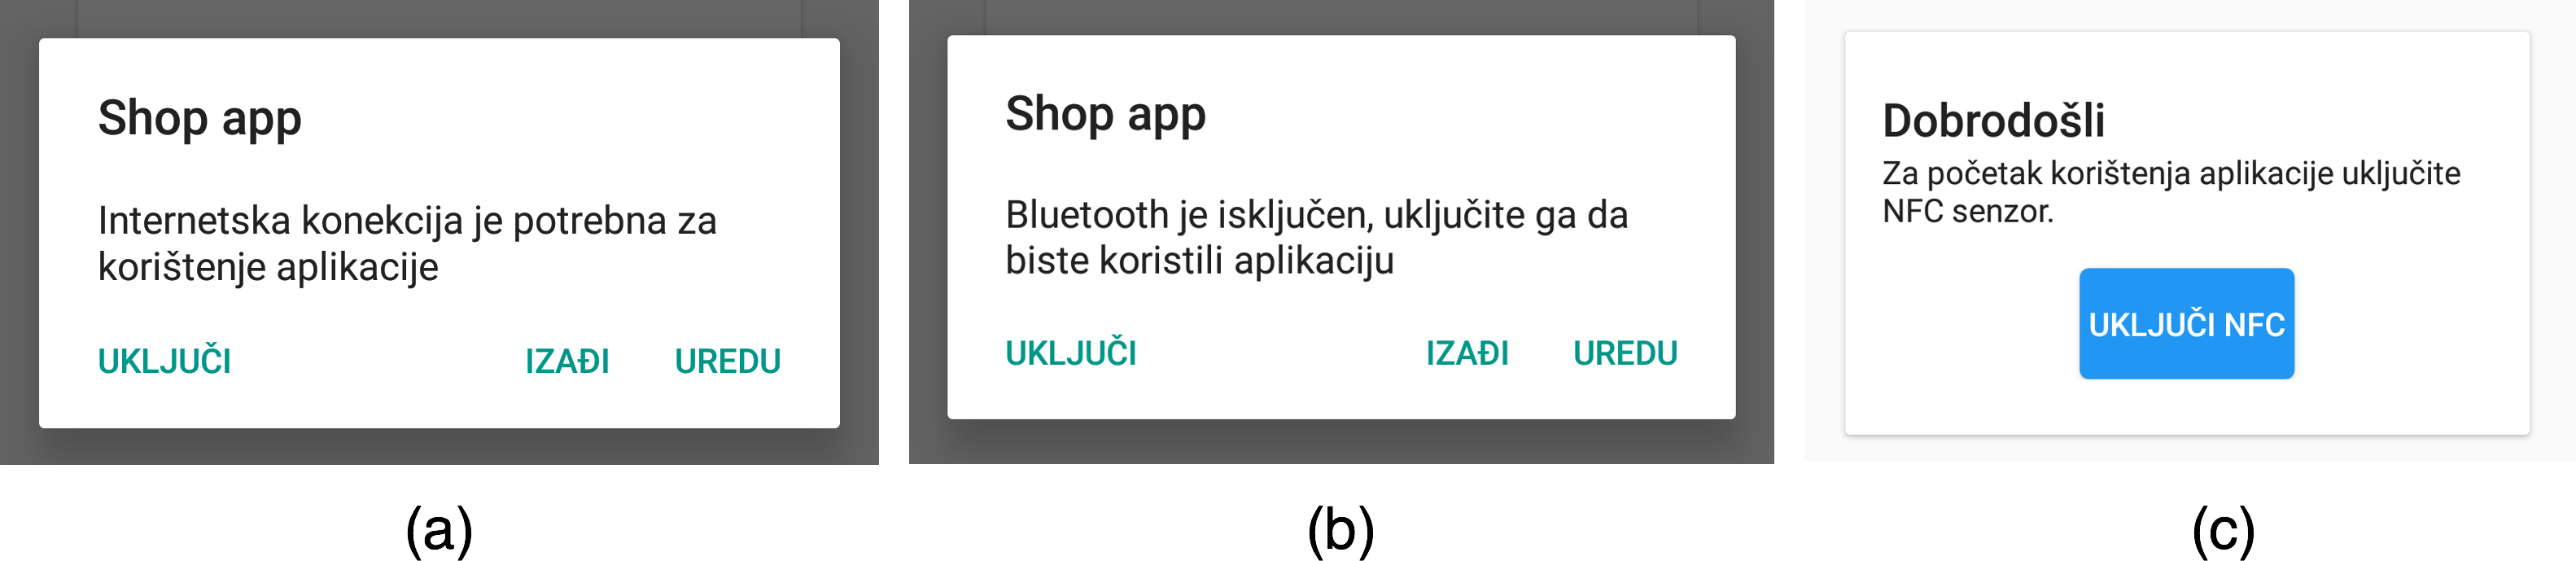
\includegraphics[height=3.3cm,keepaspectratio=true]{dijalozi}
 \caption{Obavijesti o neaktivnosti modula i akcije za uklju\v{c}ivanje istih. Obavijest (a) je vezana za Internet modul, (b) za Bluetooth modul a (c) za NFC modul}
 \label{fig:dijalozi}
	\end{center}
\end{figure}



Rukovanje isklju\v{c}enosti NFC modula je druga\v{c}ije jer je svrha po\v{c}etnog ekrana skeniranje NFC naljepnice. Stoga, ukoliko je NFC modul neaktivan, centralni dio ekrana postaje kartica s porukom u kojoj stoji da NFC modul mora biti uklju\v{c}en te tipka koja ga uklju\v{c}uje, na principu Intent-a. Jo\v{s} jedan razlog razli\v{c}ite implementacije je taj, \v{s}to su Internet i Bluetooth moduli potrebni i na svim ostalim ekranima te su ove provjere implementirane na svim ostalim ekranima, te je Dialog najjednostavnije rje\v{s}enje za implementaciju takvog zahtjeva jer se na taj na\v{c}in ne treba posebno mijenjati su\v{c}elje svakog ekrana aplikacije.

Ukoliko su svi moduli aktivni, korisniku je predstavljeno su\v{c}elje prikazano na slici \ref{fig:pocetniEkran}.


\begin{figure}[!htbp]
	\begin{center}
 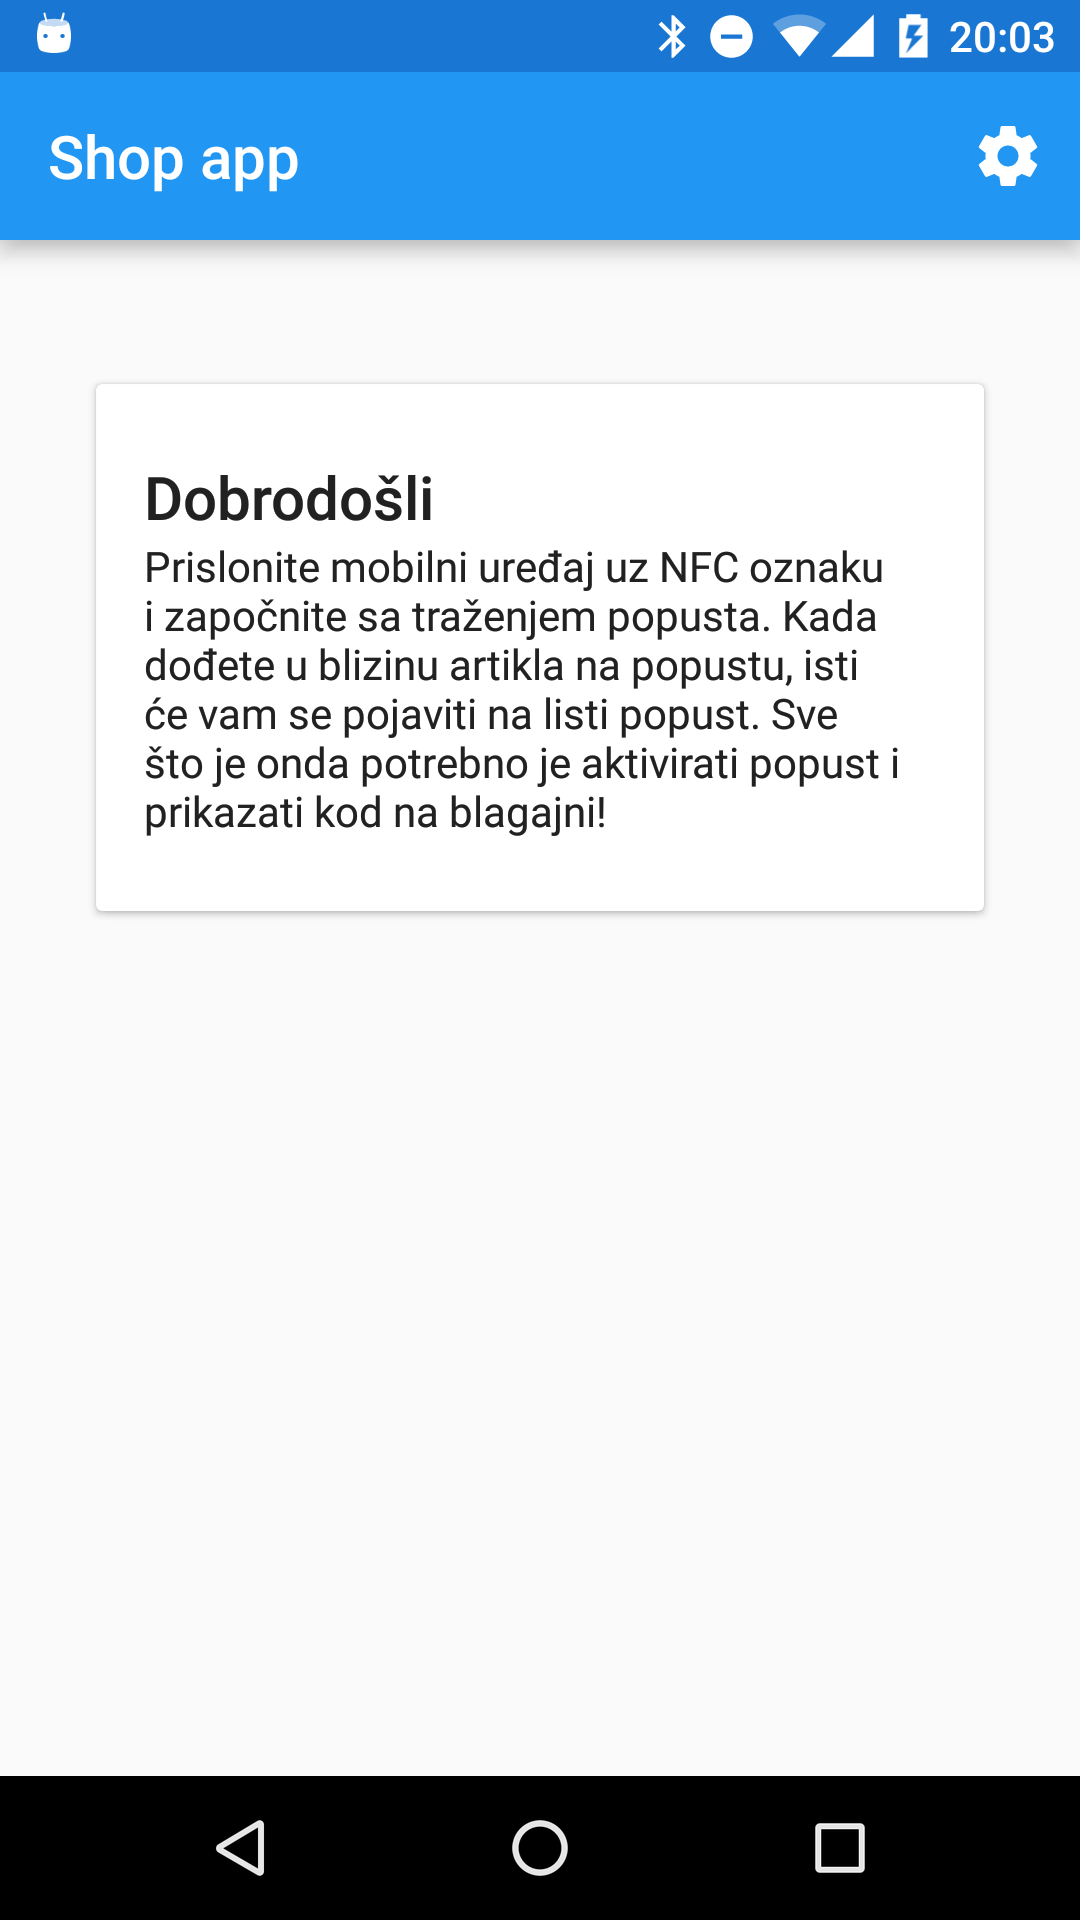
\includegraphics[height=12cm,keepaspectratio=true]{pocetni_ekran}
 \caption{Po\v{c}etni ekran}
 \label{fig:pocetniEkran}
	\end{center}
\end{figure}


\subsection{Ekran poslovnice}

Kada korisnik skenira NFC naljepnicu, otvara se ekran poslovnice i \v{c}ita se identifikacija poslovnice, pomo\'{c}u ranije opisanog mehanizma. Nakon uspje\v{s}nog \v{c}itanja identifikacije radi se zahtjev za konfiguracijom poslovnice prema poslu\v{z}itelju. Poslu\v{z}itelj vra\'{c}a osnovne informacije o poslovnici te popis popusta vezanih uz ogla\v{s}iva\v{c}e i time je zavr\v{s}en proces inicijalizacije.

Slika \ref{fig:poslovnica} prikazuje inicijalizirani ekran te dodatne informacije o poslovnici, dostupne na klik ikone informacija.



\begin{figure}[!htbp]
	\begin{center}
 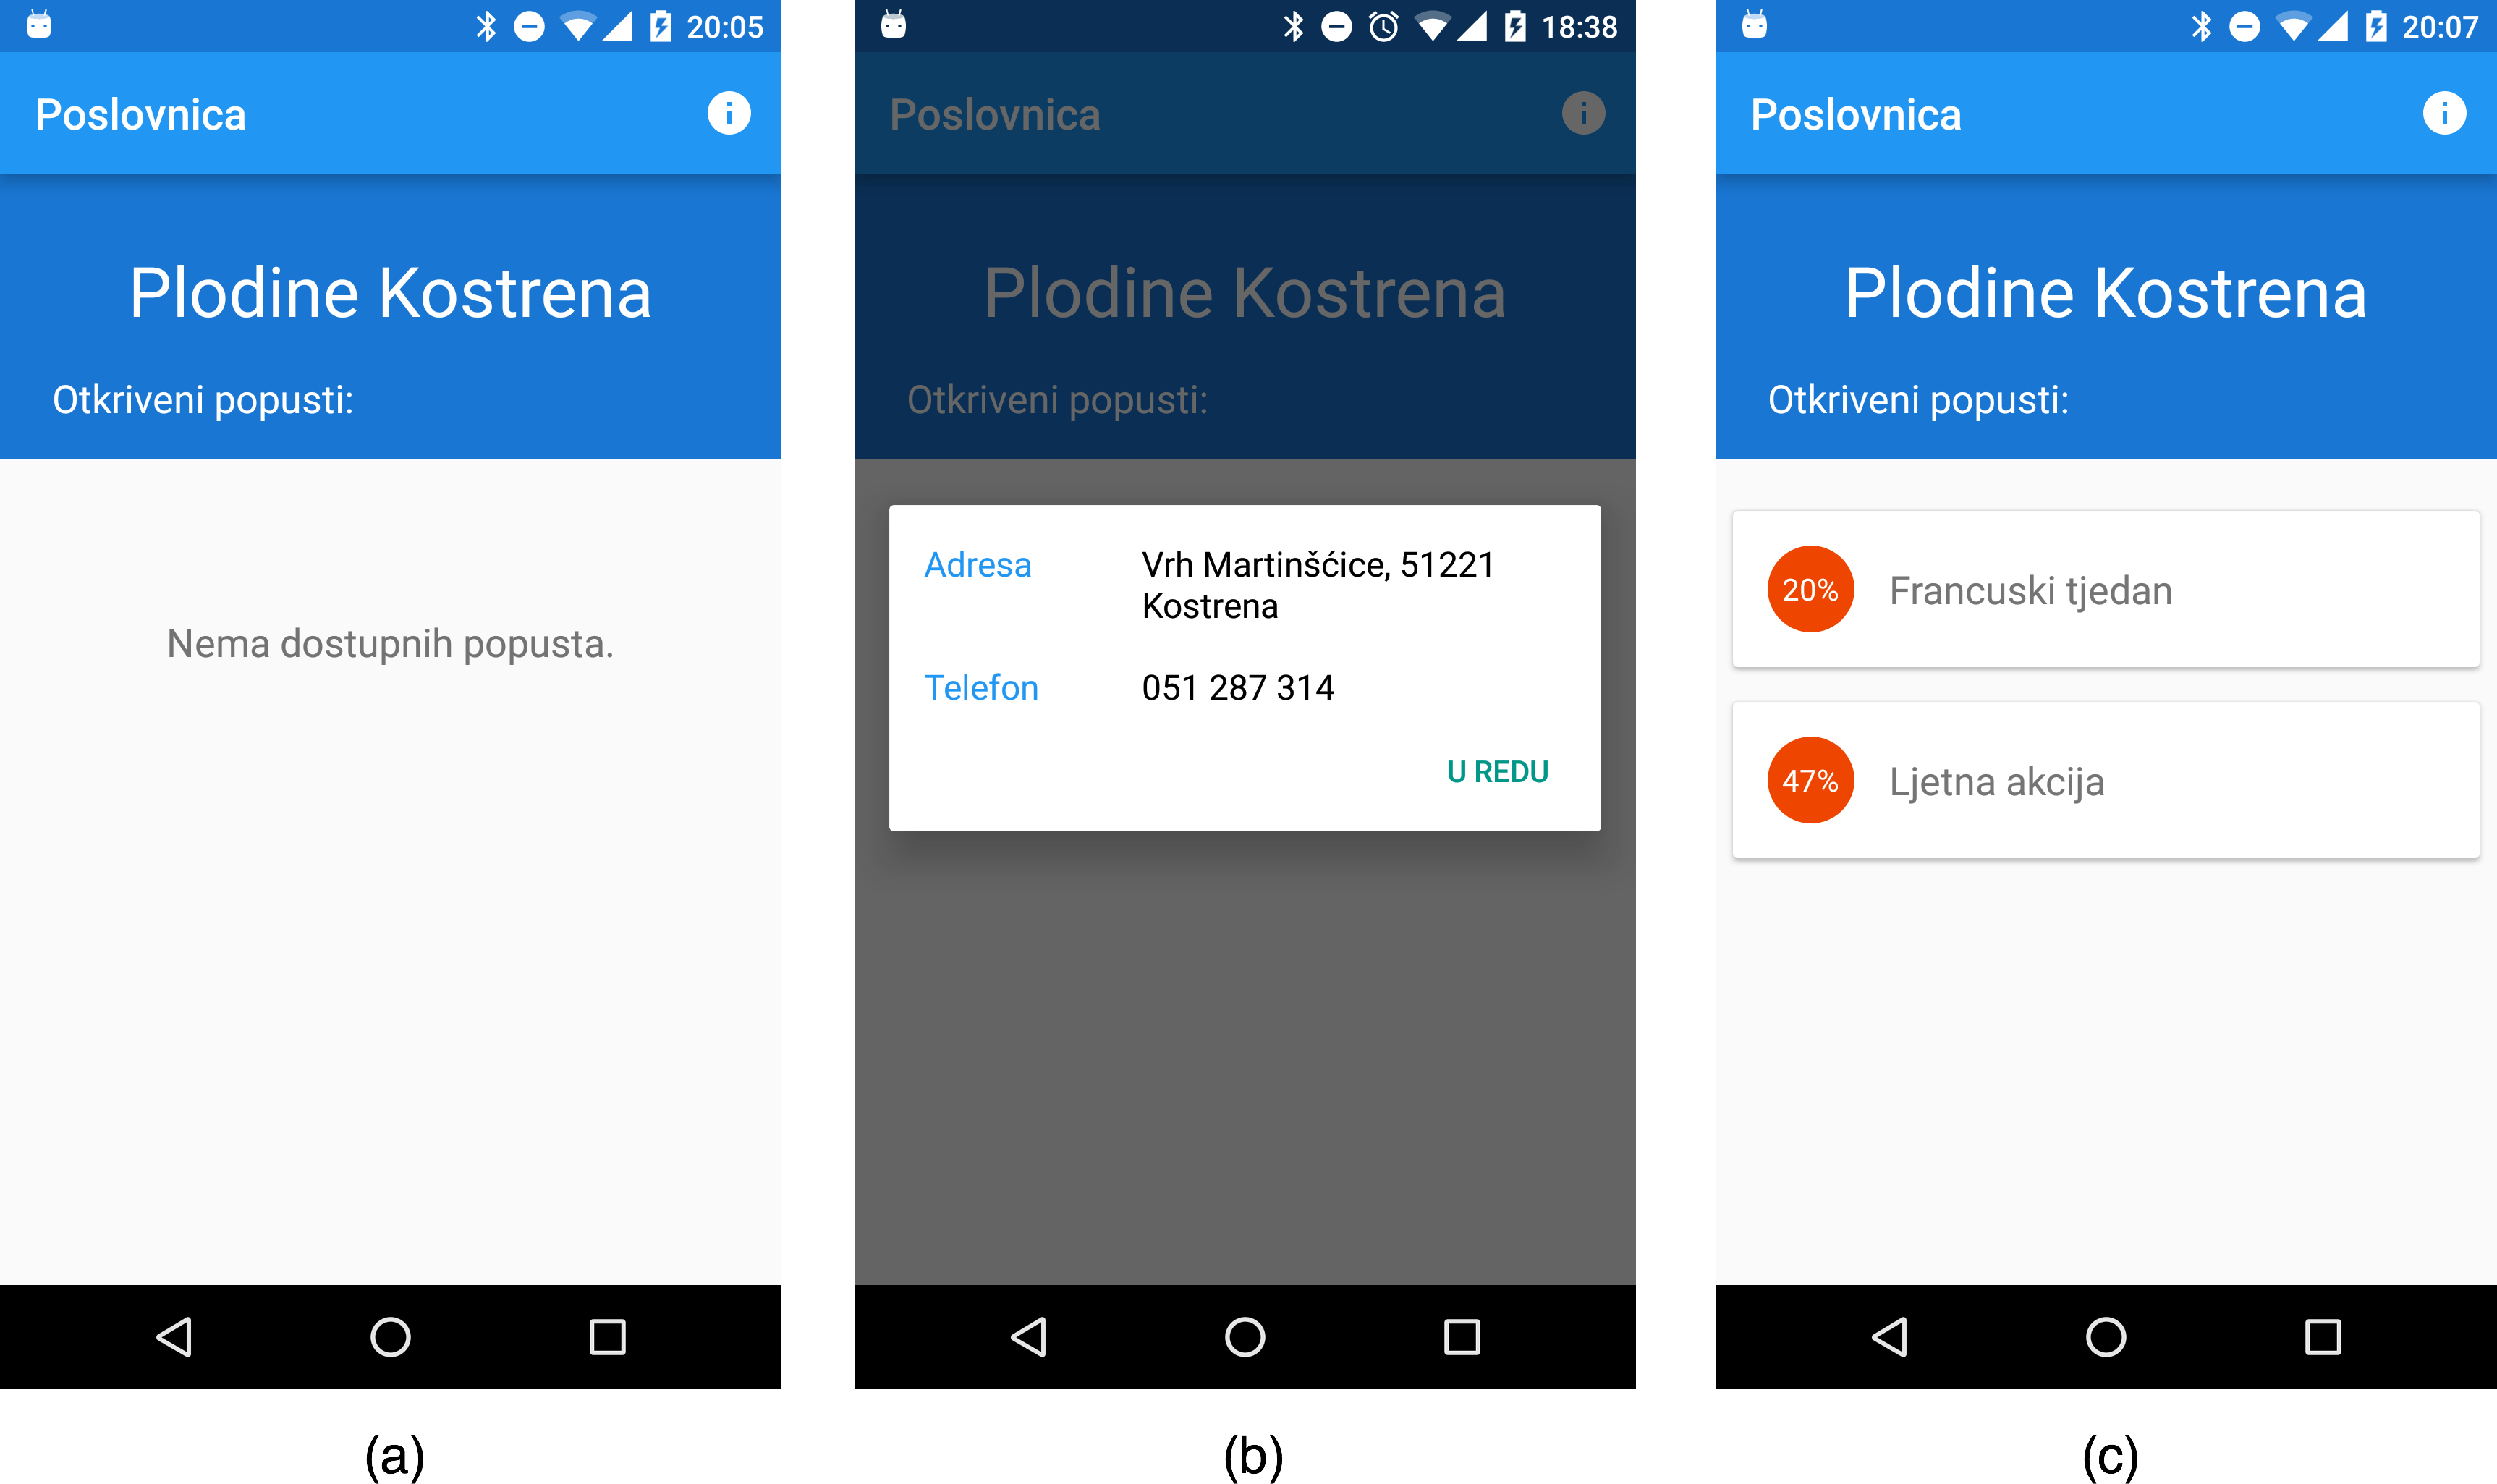
\includegraphics[height=9cm,keepaspectratio=true]{poslovnica}
 \caption{Prikaz inicijaliziranog ekrana poslovnice (a), informacija poslovnice (b) i ekrana poslovnice s otkrivenim popustima (c)}
 \label{fig:poslovnica}
	\end{center}
\end{figure}

Kada je poslovnica inicijalizirana po\v{c}inje potraga za ogla\v{s}iva\v{c}ima pomo\'{c}u opisane BLE komunikacije. Metoda za uspje\v{s}ni pronalazak ogla\v{s}iva\v{c}a poziva se svaki put kada telefon detektira ogla\v{s}iva\v{c} (konstantno se poziva dokle god je ogla\v{s}iva\v{c} u dometu telefona), te je zato implementirana logika pam\'{c}enja pronalazaka. Stoga, kada ogla\v{s}iva\v{c} bude prona\dj en prolazi se kroz popis popusta poslovnice te se uspore\dj uju zadana strojna adresa ogla\v{s}iva\v{c}a vezanog za popust i strojna adresa prona\dj enog ogla\v{s}iva\v{c}a. Ukoliko su jednake i popust jo\v{s} nije prikazan, popust se dodaje na listu popusta. Time je postignuta funkcionalnost da se korisniku puni lista popusta dok hoda kroz poslovnicu, koja je tako\dj er prikazana na slici \ref{fig:poslovnica}. Kada korisnik klikne na neki od popusta prikazuje mu se ekran detalja popusta.


\subsection{Ekran detalja popusta}

Kada korisnik prvi put otvori ekran detalja odgovaraju\'{c}eg popusta prikazani su mu detalji popusta u obliku: jedan detalj -  jedna kartica. Detalji se sastoje od imena proizvoda, stare i nove cijene, postotaka popusta i datuma isteka popusta. Ukoliko nije aktivirao popust, korisniku je predstavljen omogu\'{c}eni FAB gumb (univerzalna Android komponenta za aktiviranje glavne akcije ekrana, definirana u Material design specifikaciji \cite{materialDesign}) koji slu\v{z}i za kreiranje zahtjeva za kodom popusta. Prilikom kreiranja zahtjeva \v{c}ita se identifikator ure\dj aja (koriste\'{c}i Andorid-ovu klasu TelephonyManager \cite{telephonyManager} koja u ovisnosti o dostupnosti vra\'{c}a IMEI, MEID ili ESN broj koji je jednozna\v{c}an za svaki ure\dj aj) s ciljem ograni\v{c}avanja izdanih kodova na jedan po ure\dj aju. Ukoliko je zahtjev uspje\v{s}an korisnik je o tome obavje\v{s}ten odgovaraju\'{c}om porukom te mu se na detaljima popusta pojavljuje nova kartica koja sadr\v{z}i kod kojeg je du\v{z}an prikazati na blagajni. Na slici \ref{fig:detalji_poslovnice} je prikazan opisan ekran i stanja u kojima se mo\v{z}e nalaziti.



\begin{figure}[!htbp]
	\begin{center}
 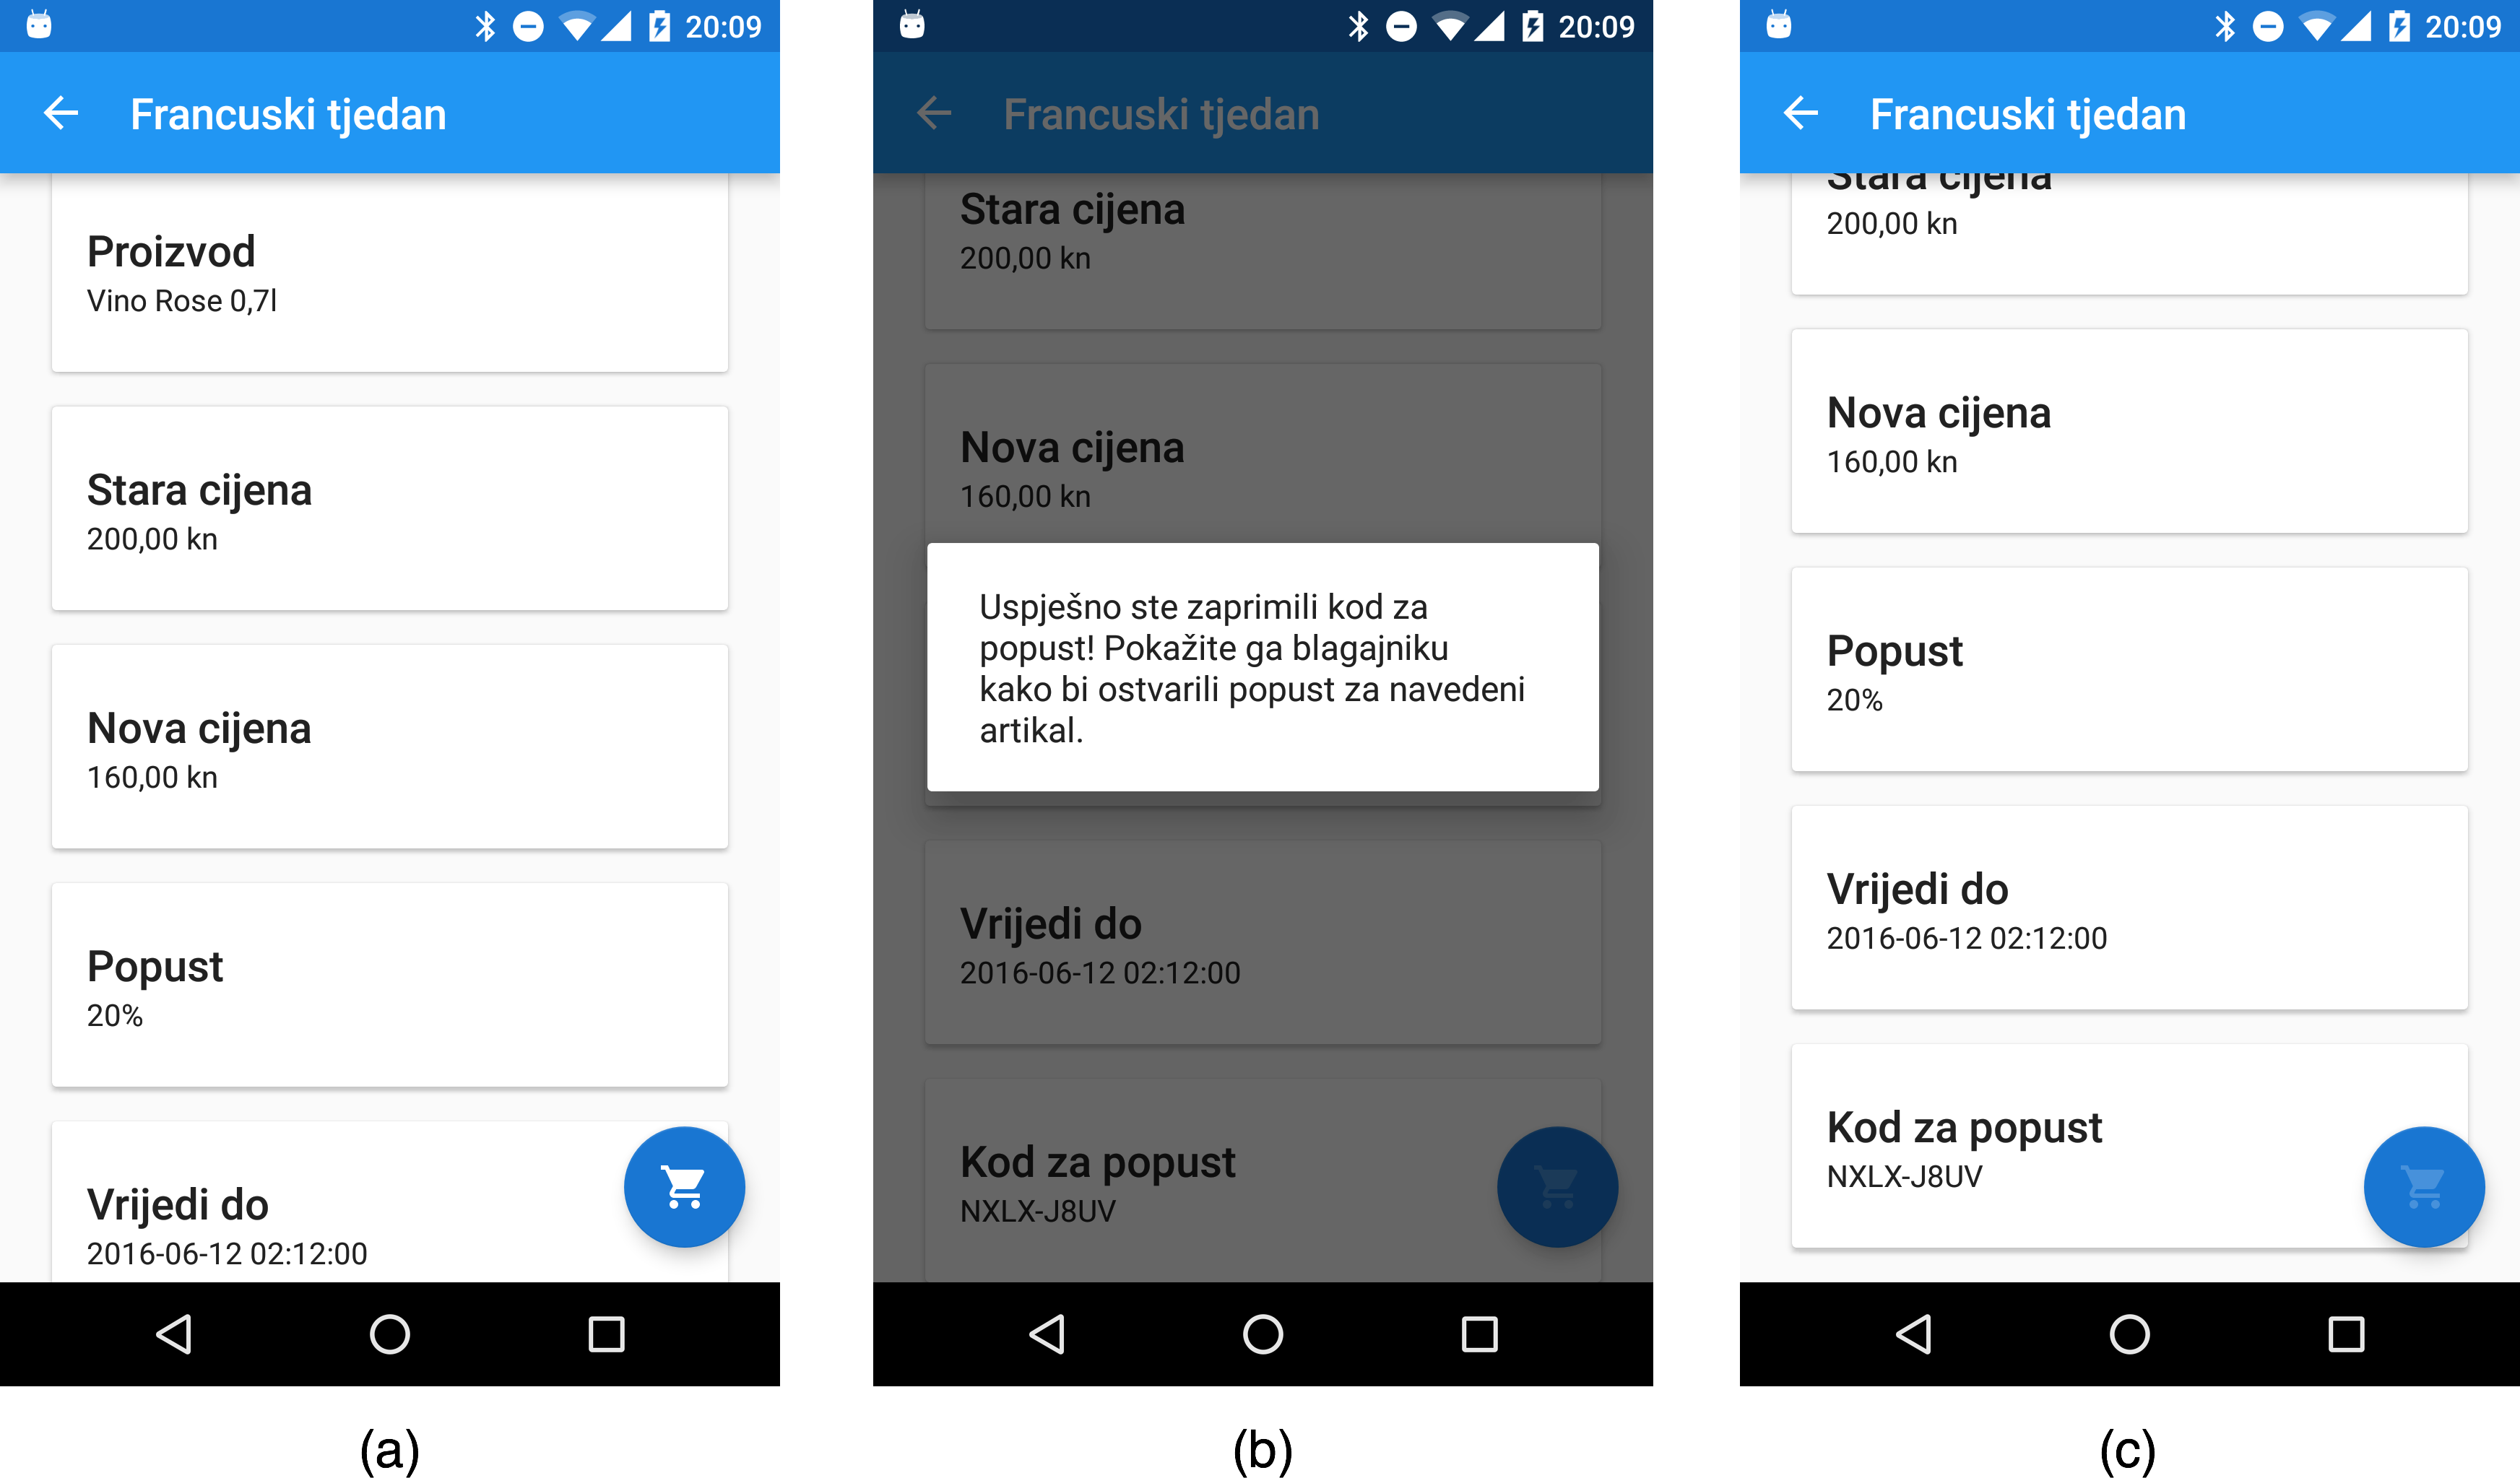
\includegraphics[height=9cm,keepaspectratio=true]{detalji_poslovnice}
 \caption{Slika sadr\v{z}i prikaz inicijalnog ekrana sa detaljima popusta (a), poruka uspje\v{s}nog primanja koda (b) i ekran sa detaljima popusta koji uklju\v{c}uje i kod za popust (c)}
 \label{fig:detalji_poslovnice}
	\end{center}
\end{figure}


\subsection{Ekran postavki}
Ekran popusta sadr\v{z}i opciju za postavljanje gornje granice ja\v{c}ine signala BLE ogla\v{s}iva\v{c}a koja je dovoljna da aplikacija detektira ogla\v{s}iva\v{c}. Granica ozna\v{c}ava numeri\v{c}ku vrijednost u decibelima te se prilikom detekcije BLE ogla\v{s}iva\v{c}a evaluira vrijednost detekiranog signala te, ukoliko je unutar unutrar zadane granice, aplikacija nastavlja sa obra\dj ivanjem BLE ogla\v{s}iva\v{c}a.
Odabrana numeri\v{c}ka vrijednost se zapisuje u internu memoriju pametnog telefona te ona ostaje dostupna i nakon \v{s}to aplikacija prestane sa radom. Slika \ref{fig:postavke} prikazuje ekran postavki.


\begin{figure}[!htbp]
	\begin{center}
 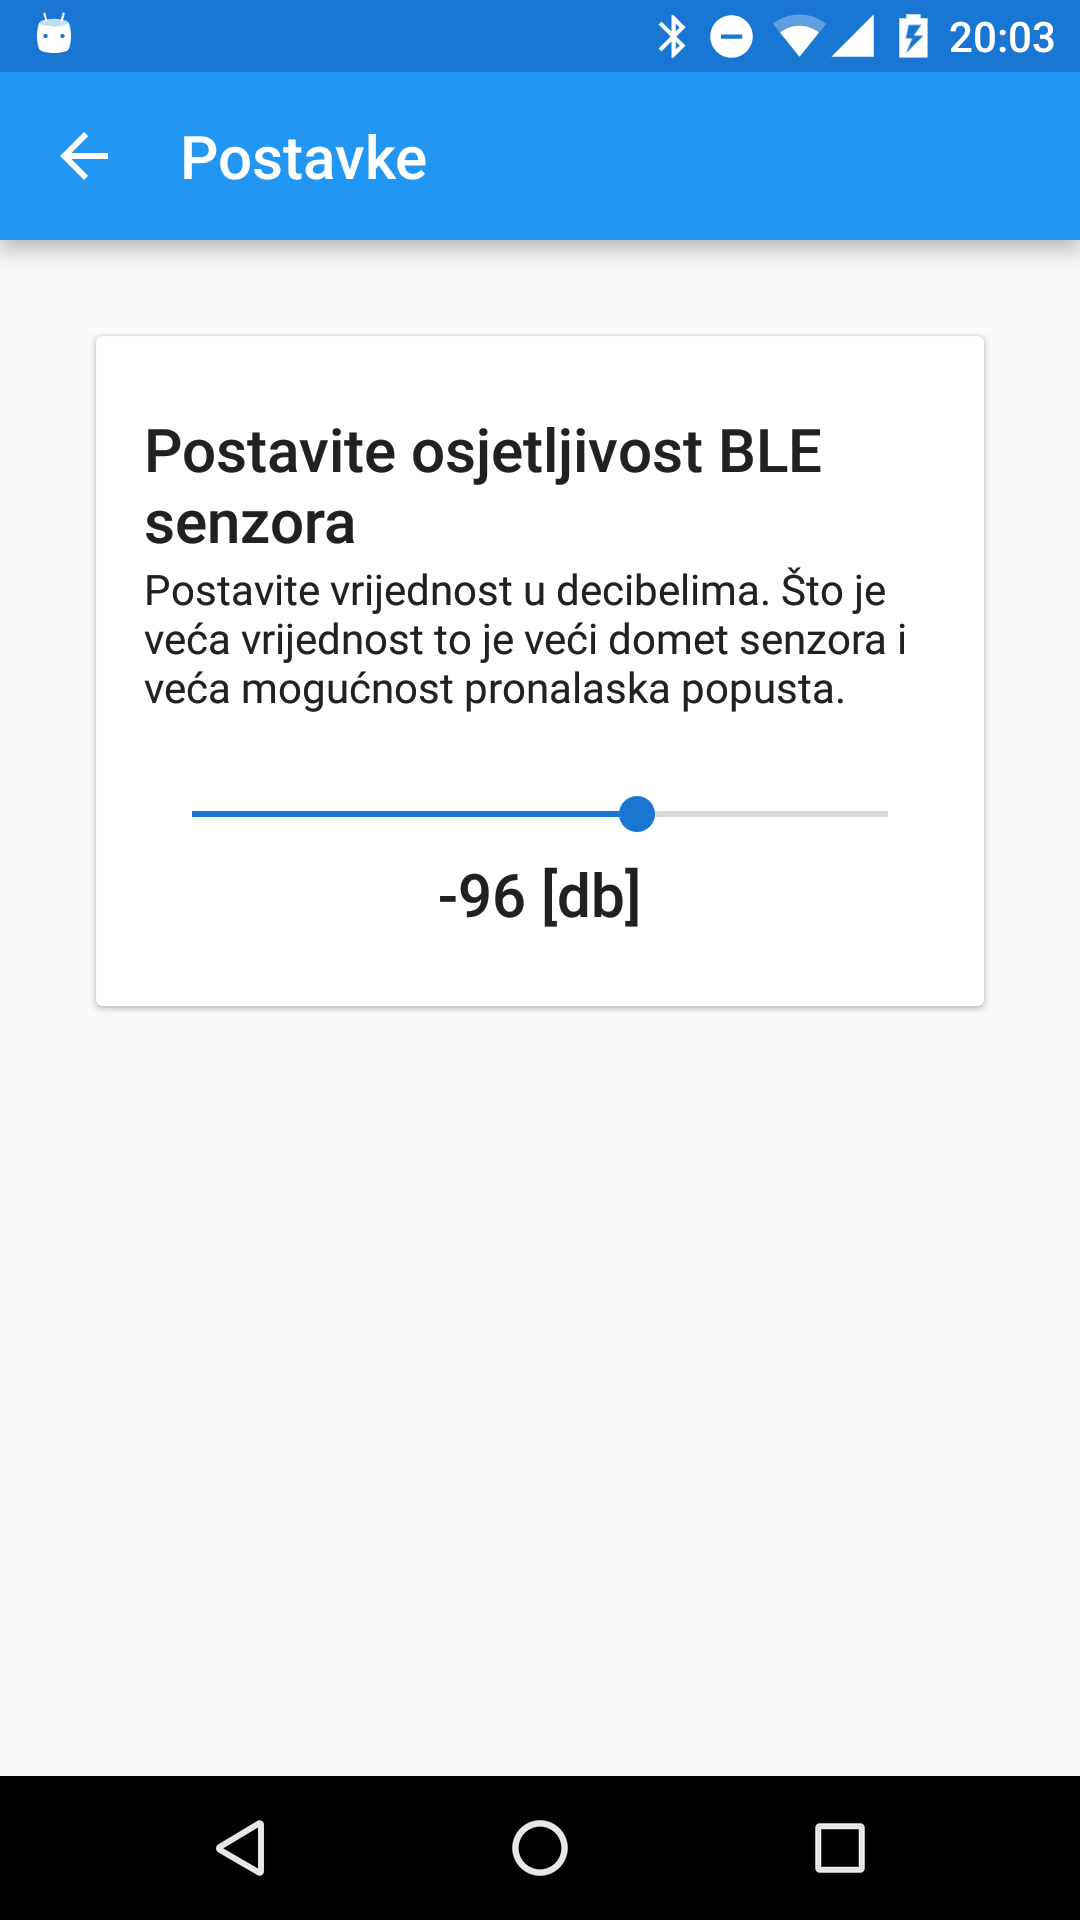
\includegraphics[height=12cm,keepaspectratio=true]{postavke}
 \caption{Ekran postavki u kojemu je korisniku dopu\v{s}teno odabrati gornju granicu ja\v{c}ine signala, dovoljnog za detekciju od strane aplikacije}
 \label{fig:postavke}
	\end{center}
\end{figure}


\section{Kori\v{s}tene knji\v{z}nice}

Knji\v{z}nica ozna\v{c}ava skup resursa koji se dodaju u izvorni kod projekta, a slu\v{z}e za pru\v{z}anje odre\dj enih funkcionalnosti. Uklju\v{c}ivanjem knji\v{z}nica u projekt se mo\v{z}e bitno skratiti vrijeme potrebno za razvoj jer nije potrebno implementirati ne\v{s}to \v{s}to je ve\'{c} implementirano, dobro testirano i stavljeno na tr\v{z}i\v{s}te. S druge strane, dodavanjem knji\v{z}nice se dobivaju sve njene funkcionalnosti koje mogu pove\'{c}ati veli\v{c}inu projekta (potencijalni problem kod Androida jer korisnici ne preferiraju aplikacije koje zauzimaju puno memorije).
Dodavanje knji\v{z}nica se u Android-u se radi preko Gradle priklju\v{c}ka \cite{gradle} koji slu\v{z}i za izgradnju projekta. Proces dodavanja knji\v{z}nice uklju\v{c}uje upis lokacije knji\v{z}nice u datoteku build.gradle (konfiguracijska datoteka zapisana u programskom jeziku Groovy \cite{groovy}, koja definira izgradnju projekta). Lokacija knji\v{z}nice je zapravo ime paketa i verzija \v{z}eljene knji\v{z}nice, \v{s}to je dovoljno informacija Gradle priklju\v{c}ku da je prona\dj e na repozitoriju jCenter \cite{jcenter} (centralni repozitor za Android knji\v{z}nice otvorenog koda) i preuzme. Tada kod knji\v{z}nice postaje dostupan za kori\v{s}tenje u cijelom projektu.
Kori\v{s}tene knji\v{z}nice su:

\begin{itemize}
	\item Support design
	\begin{itemize}
		\item Google-ova slu\v{z}bena knji\v{z}nica u kojoj se nalaze komponente korisni\v{c}kog su\v{c}elja te se pru\v{z}a kompatibilnost za stare verzije Android-a
	\end{itemize}

	\item Okhttp \cite{okhttp}
	\begin{itemize}
		\item HTTP klijent za Android i Java aplikacije
		\item Koristi se za komunikaciju aplikacije sa poslu\v{z}iteljom
	\end{itemize}

	\item GSON \cite{gson}
	\begin{itemize}
		\item Knji\v{z}nica za serijalizaciju JSON objekata u Java objekte i obrnuto
		\item Koristi se serijalizaciju odgovora poslu\v{z}itelja u model
	\end{itemize}
	
	\item Butterknife \cite{butterKnife}
	\begin{itemize}
		\item Knji\v{z}nica koja uvodi anotacije koje povezuju komponentu korisni\v{c}kog su\v{c}elja definiranog u XML-u sa Java objektom, preko identifikatora
		\item Koristi se za smanjivanje linija koda i \v{c}i\v{s}\'{c}i kod
	\end{itemize}


	\item EventBus \cite{eventBus}
	\begin{itemize}
		\item Knji\v{z}nica za ogla\v{s}avanje i pretplatu na doga\dj aje
		\item Slu\v{z}i za olak\v{s}avanje komunikacije izme\dj u klasa
		\item Koristi se za obavijest o promjeni stanja BLE i internet modula na razini cijele aplikacije
	\end{itemize}
\end{itemize}

